% ============================================================
% MemUpdateBench — Production Manuscript
% To switch to ACL/EMNLP format:
%   1. Replace \documentclass and geometry with the venue .sty
%   2. Keep all \section / \table / \figure commands unchanged
% ============================================================
\documentclass[11pt,twocolumn]{article}

\usepackage[margin=1in]{geometry}
\usepackage{times}
\usepackage{graphicx}
\usepackage{booktabs}
\usepackage{multirow}
\usepackage{amsmath}
\usepackage{url}
\usepackage[numbers,sort&compress]{natbib}
\usepackage{xcolor}

\graphicspath{{figures/}}

\title{MemUpdateBench: How Stale Context Contaminates\\Memory-Augmented LLM Answering}
\author{Anonymous Authors}
\date{}

\begin{document}
\maketitle

% ============================================================
% ABSTRACT  (~170 words)
% ============================================================
\begin{abstract}
When a user tells an LLM agent ``I moved to Tokyo,'' the agent should update its external memory---but what happens to the old entry ``lives in Paris''?
We show that lingering obsolete entries silently contaminate the answer-time context and cause catastrophic accuracy loss.
On MemUpdateBench, a controlled diagnostic benchmark that stresses the same \((\text{entity},\text{attribute})\) slot with up to 16 repeated updates, append-only memory preserves the correct final value yet collapses to 0.07 EM under prompted answering, because 14 stale same-slot entries overwhelm the context.
A single retrieved stale entry halves accuracy; two push it below 20\%.
Through synthetic probes we identify the mechanism as an interaction of \emph{version ambiguity} and \emph{positional bias} rather than simple majority voting: explicit version labels almost fully repair the failure.
Across three model families (Qwen, Llama, Mistral), retrieval-time stale filtering recovers each model to its own zero-stale ceiling, confirming stale context as the dominant answer-layer obstacle.
These findings imply that memory systems must actively manage obsolete entries, not merely accumulate evidence.
\end{abstract}

% ============================================================
% §1  INTRODUCTION
% ============================================================
\section{Introduction}

External memory gives language-model agents a way to carry user preferences, facts, and task state across sessions.
Most evaluation settings ask whether a system can \emph{retrieve} a relevant fact after it has been stored.
In realistic use, however, the same fact is revised repeatedly: a user moves cities, switches jobs, updates a project deadline, or corrects an earlier statement.
Each revision overwrites the intended slot value, but many memory implementations simply \emph{append} the new evidence without removing the old.
The result is a growing pool of obsolete entries that coexist with the current value.

Does this matter?  Under oracle slot lookup the answer is no: the correct value is still there.
Under prompted answering---where the model must select the right value from a retrieved context that may contain both current and obsolete entries---the answer is a decisive yes.
On our controlled benchmark, append-only memory maintains perfect state recoverability at \(k{=}16\) updates yet collapses to 0.07~EM under slot-conditioned answering.
A retrieval-time stale filter that exposes only the latest entry per slot recovers EM from 0.14 to 0.69---matching the zero-stale oracle ceiling.

This paper asks three questions:
\begin{enumerate}
\item \textbf{Dominance.}  Is stale same-slot context the dominant answer-layer obstacle, or do other factors contribute comparably?
\item \textbf{Mechanism.}  What drives stale-induced answer collapse---majority voting, positional bias, version ambiguity, or their interaction?
\item \textbf{Generality.}  Are these findings specific to one model, or do they hold across architectures?
\end{enumerate}

To answer these questions we introduce MemUpdateBench, a diagnostic benchmark that isolates repeated same-slot updates with controlled update frequency~\(k\), same-name distractors, and semantic near-miss events.
The benchmark reports four quantities that are often conflated: final-state reliability, stale same-slot burden, memory compactness, and slot-conditioned answer robustness.
This multi-axis design lets us separate storage-layer failures from answer-layer failures.

Our findings are:
(1)~Stale context is the dominant answer-layer obstacle: filtering it recovers each of three tested models to its own zero-stale ceiling (Table~\ref{tab:ceiling-recovery}).
(2)~The mechanism is an interaction of version ambiguity and positional bias; explicit version labels almost completely repair the failure even with 16~conflicting stale entries.
(3)~The collapse generalizes across Qwen, Llama, and Mistral, while the absolute recovery level reflects each model's prompt-following capacity rather than differential stale susceptibility.

MemUpdateBench is complementary to broad agent-memory benchmarks such as LoCoMo~\citep{locomo} and LongMemEval~\citep{longmemeval}, which emphasize ecological validity.
Our benchmark is narrower by design: it makes one failure pressure---stale same-slot contamination---precisely measurable.\footnote{Code and data will be released upon acceptance.}

% ============================================================
% §2  BENCHMARK
% ============================================================
\section{MemUpdateBench}

\paragraph{Slot structure.}
Each example defines a target slot \((\text{entity}, \text{attribute})\) with a gold final value.
Events take one of three actions: \textsc{Add} introduces a new slot value, \textsc{Update} revises an existing value, and \textsc{Noop} mentions the entity or attribute without changing the slot.
This exact structure lets us compute both whether the final value is recoverable and how many obsolete same-slot values remain.

\paragraph{Update frequency as independent variable.}
The main split varies \(k \in \{1,2,4,8,16\}\), where \(k\) is the number of times the target slot is written.
Larger~\(k\) means more stale same-slot entries for non-compacting memory.
This controlled axis directly stresses whether a memory system overwrites obsolete values or lets them accumulate.

\paragraph{Hard distractors.}
The hard split includes same-name multi-entity distractors (another person with the same first name) and semantic near-miss \textsc{Noop} events (``discussed Python in a workshop'' when the target attribute is \emph{programming language}).
Success therefore requires resolving the intended entity \emph{and} attribute rather than reacting to surface lexical overlap.

\paragraph{Scope.}
The benchmark is intentionally narrow.
It covers explicit key-value slot updates and does not attempt to model implicit updates, negations, or conditional revisions.
This controlled scope is both a strength---it makes stale burden precisely measurable---and a limitation acknowledged in \S\ref{sec:limitations}.

% ============================================================
% §3  EXPERIMENTAL SETUP
% ============================================================
\section{Experimental Setup}

\paragraph{Memory managers.}
We compare four systems that span the reliability--compactness spectrum:
\textbf{Constrained CRUD} performs exact slot-level updates and deletes stale entries by construction; it is an oracle-like diagnostic upper bound, not a deployable system.
\textbf{Raw append} keeps every observed event, making stale burden maximally visible.
\textbf{Heuristic CRUD} applies rule-based partial compaction.
\textbf{Long25} is a learned compact manager from a constrained-slot curriculum; it is included as a compactness--reliability tradeoff point.

\paragraph{Answer modes.}
\texttt{slot\_direct} checks whether the final value can be resolved by exact slot lookup (oracle-like state evaluation).
\texttt{slot\_prompt} asks the model to answer a slot-conditioned question using the memory contents as context.
The gap between these two modes is central to the paper.

\paragraph{Metrics.}
We report four quantities together:
(1)~state accuracy under \texttt{slot\_direct},
(2)~EM/F1 under \texttt{slot\_prompt},
(3)~stale same-slot entry count, and
(4)~final memory size.
No single metric suffices: state accuracy can hide stale evidence, EM/F1 can conflate state and answer failures, and memory size alone can reward over-deletion.

\paragraph{Answer models.}
We evaluate three instruction-tuned models at the 7--8B scale: Qwen2.5-7B-Instruct~\citep{qwen25}, Llama-3.1-8B-Instruct~\citep{llama31}, and Mistral-7B-Instruct~\citep{mistral}.

% ============================================================
% §4  STALE CONTAMINATION AND RECOVERY
% ============================================================
\section{Stale Contamination and Recovery}

\subsection{State accuracy masks answer collapse}

One might expect that a memory system which never loses the final value would also answer correctly.
Under oracle-like \texttt{slot\_direct} evaluation, this expectation holds: Constrained CRUD, Raw append, and Heuristic CRUD all maintain state accuracy 1.00 through \(k{=}16\) (Figure~\ref{fig:p63-update-frequency-tradeoff}).
The final value is always recoverable.

\begin{figure}[t]
  \centering
  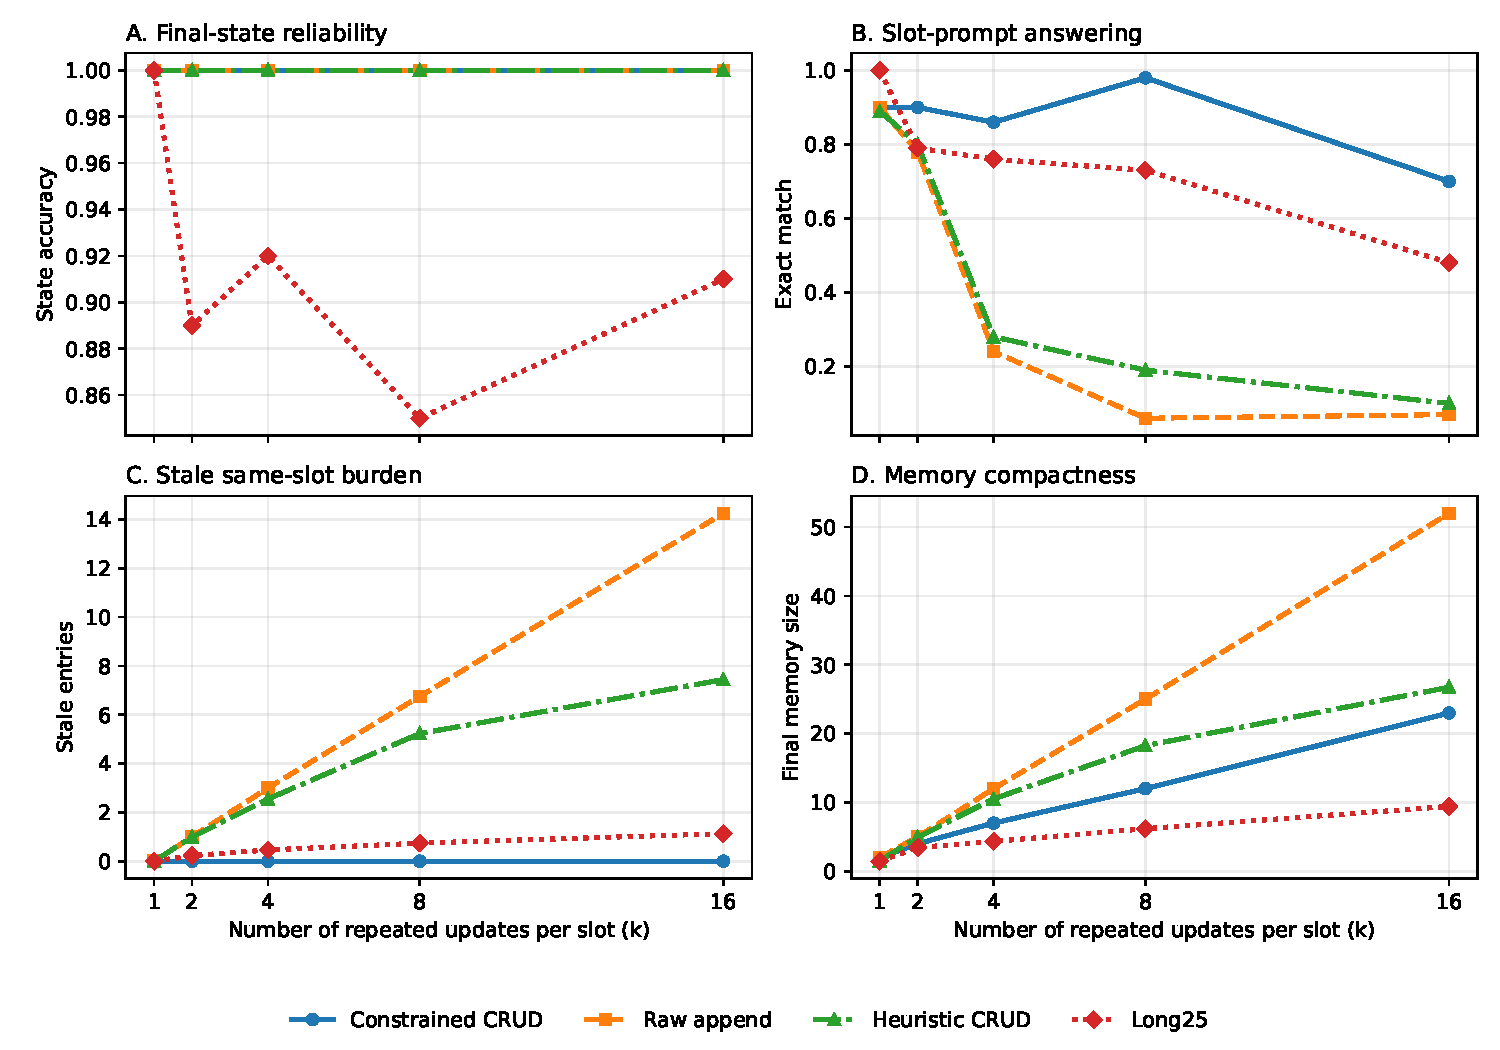
\includegraphics[width=\linewidth]{figures/p63_update_frequency_tradeoff.pdf}
  \caption{Update-frequency stress test on the hard split. \texttt{slot\_direct} state accuracy (left) hides stale burden; \texttt{slot\_prompt} EM (right) reveals answer collapse as \(k\) grows.}
  \label{fig:p63-update-frequency-tradeoff}
\end{figure}

But under \texttt{slot\_prompt} answering, append-style memory collapses catastrophically.
Raw append falls from 0.90~EM at \(k{=}1\) to \textbf{0.07~EM} at \(k{=}16\) on the hard test split, while retaining 14.25 stale same-slot entries and a final memory size of~52.
The correct value is still in memory---the model simply cannot find it amid the obsolete alternatives.
Table~\ref{tab:p63-k16-tradeoff} shows the full \(k{=}16\) tradeoff.

\begin{table}[t]
\centering
\small
\begin{tabular}{lrrrr}
\toprule
Method & State & EM / F1 & Stale & Mem. \\
\midrule
Constrained CRUD & 1.00 & .70 / .70 & 0.0 & 23 \\
Raw append       & 1.00 & .07 / .10 & 14.3 & 52 \\
Heuristic CRUD   & 1.00 & .10 / .13 & 7.4 & 27 \\
Long25           & 0.91 & .48 / .53 & 1.1 & 9 \\
\bottomrule
\end{tabular}
\caption{High-frequency \(k{=}16\) tradeoff (hard test). State accuracy alone hides stale burden; append-only memory collapses under prompted answering despite perfect state.}
\label{tab:p63-k16-tradeoff}
\end{table}

\subsection{Stale filtering as diagnostic intervention}

If stale same-slot entries are truly the dominant obstacle, removing them at retrieval time should recover answer accuracy---without changing anything about the stored memory.

We test this with a \emph{latest-per-slot} intervention: raw-append writes are unchanged, but at answer time we expose only the most recent entry for each slot.
On \(k{=}16\) dev, this raises EM from 0.14 to \textbf{0.69}---a gain of \(+0.55\)---while stale retrieved entries drop from 4.04 to~0.
The same pattern holds across update frequencies: latest-per-slot maintains strong EM even as \(k\) grows (expanded split \(k{=}16\): EM 0.750).

Crucially, the recovered EM (0.69) closely matches the zero-stale Constrained CRUD ceiling (0.70).
This means the stale filter accounts for nearly \emph{all} of the stale-specific answer loss.

\subsection{Three-model ceiling recovery}

Is this finding model-specific?
We replicate the stale collapse and latest-per-slot recovery on Llama-3.1-8B and Mistral-7B.
For each model we also run a zero-stale Constrained CRUD control to establish the model's own clean-memory ceiling.

\begin{table}[t]
\centering
\small
\begin{tabular}{lrrrr}
\toprule
Model & Normal & Filtered & Ceiling & Gap \\
\midrule
Qwen2.5-7B   & .110 & .690 & .700 & $-.01$ \\
Llama3.1-8B  & .060 & .290 & .270 & $+.02$ \\
Mistral-7B   & .080 & .720 & .720 & $.00$ \\
\bottomrule
\end{tabular}
\caption{Ceiling recovery on \(k{=}16\) dev. \emph{Normal}: raw-append top-\(k\) retrieval. \emph{Filtered}: latest-per-slot. \emph{Ceiling}: zero-stale Constrained CRUD \texttt{slot\_prompt}. \emph{Gap}: Filtered $-$ Ceiling. All three models recover to within 0.02~EM of their own zero-stale ceiling.}
\label{tab:ceiling-recovery}
\end{table}

Table~\ref{tab:ceiling-recovery} shows the result: all three models collapse under stale-contaminated retrieval (\({\leq}0.11\)~EM), and all three recover to within 0.02~EM of their own zero-stale ceiling after stale filtering.
The absolute EM levels differ---Llama's ceiling is 0.27 while Qwen's and Mistral's are near 0.70---but the \emph{stale-specific} loss is removed in every case.
The remaining differences reflect each model's prompt-following and context-utilization capacity, not a differential stale mechanism.

This is the paper's central result: \textbf{stale same-slot contamination is the dominant answer-layer obstacle for all tested models}, and retrieval-time stale filtering is sufficient to recover each model to its clean-memory ceiling.

% ============================================================
% §5  MECHANISM ANALYSIS
% ============================================================
\section{Mechanism Analysis}

The ceiling-recovery result (\S4) establishes \emph{that} stale context is the dominant obstacle.
This section asks \emph{why} stale entries break answer generation, using four complementary probes.

\subsection{Context presentation sensitivity}
\label{sec:context-presentation}

We first ask whether the \emph{way} stale entries are presented matters, holding their composition fixed.
In real raw-append \(k{=}16\) dev contexts, gold retrieval rate (0.360) and retrieved stale count (4.04) are identical across all conditions below; only presentation changes.

\begin{table}[t]
\centering
\small
\begin{tabular}{lrr}
\toprule
Presentation & EM & F1 \\
\midrule
Normal (default) & .110 & .136 \\
Chronological order & .230 & .275 \\
Reverse chronological & .010 & .050 \\
Timestamp labels & .150 & .200 \\
Latest / outdated labels & .260 & .298 \\
\bottomrule
\end{tabular}
\caption{Real-context presentation probe (\(k{=}16\) dev, Qwen). Retrieved composition is fixed across rows; only presentation changes. Chronological and explicit labels improve EM; reverse chronological nearly destroys it.}
\label{tab:real-context-mechanism}
\end{table}

Table~\ref{tab:real-context-mechanism} shows large effects.
Chronological ordering roughly doubles EM (0.11\(\to\)0.23), while reverse chronological nearly eliminates it (0.01).
Explicit \texttt{[latest]}/\texttt{[outdated]} labels improve EM to 0.26.
Because retrieval composition is identical, these differences are purely answer-layer: the model is sensitive to \emph{where} the current value appears and \emph{whether} version information is explicit.

\subsection{Isolating the mechanism: conflict, order, and labels}
\label{sec:synthetic-probe}

Real contexts confound stale count with other retrieval variables.
We therefore construct synthetic same-slot probes with exact control over three factors:
(1)~whether stale values \emph{conflict} with the current value or repeat it,
(2)~context \emph{order} (chronological vs.\ reverse chronological), and
(3)~whether entries carry explicit \texttt{[latest]}/\texttt{[outdated]} \emph{labels}.
Each cell contains 64~examples.

\begin{figure}[t]
  \centering
  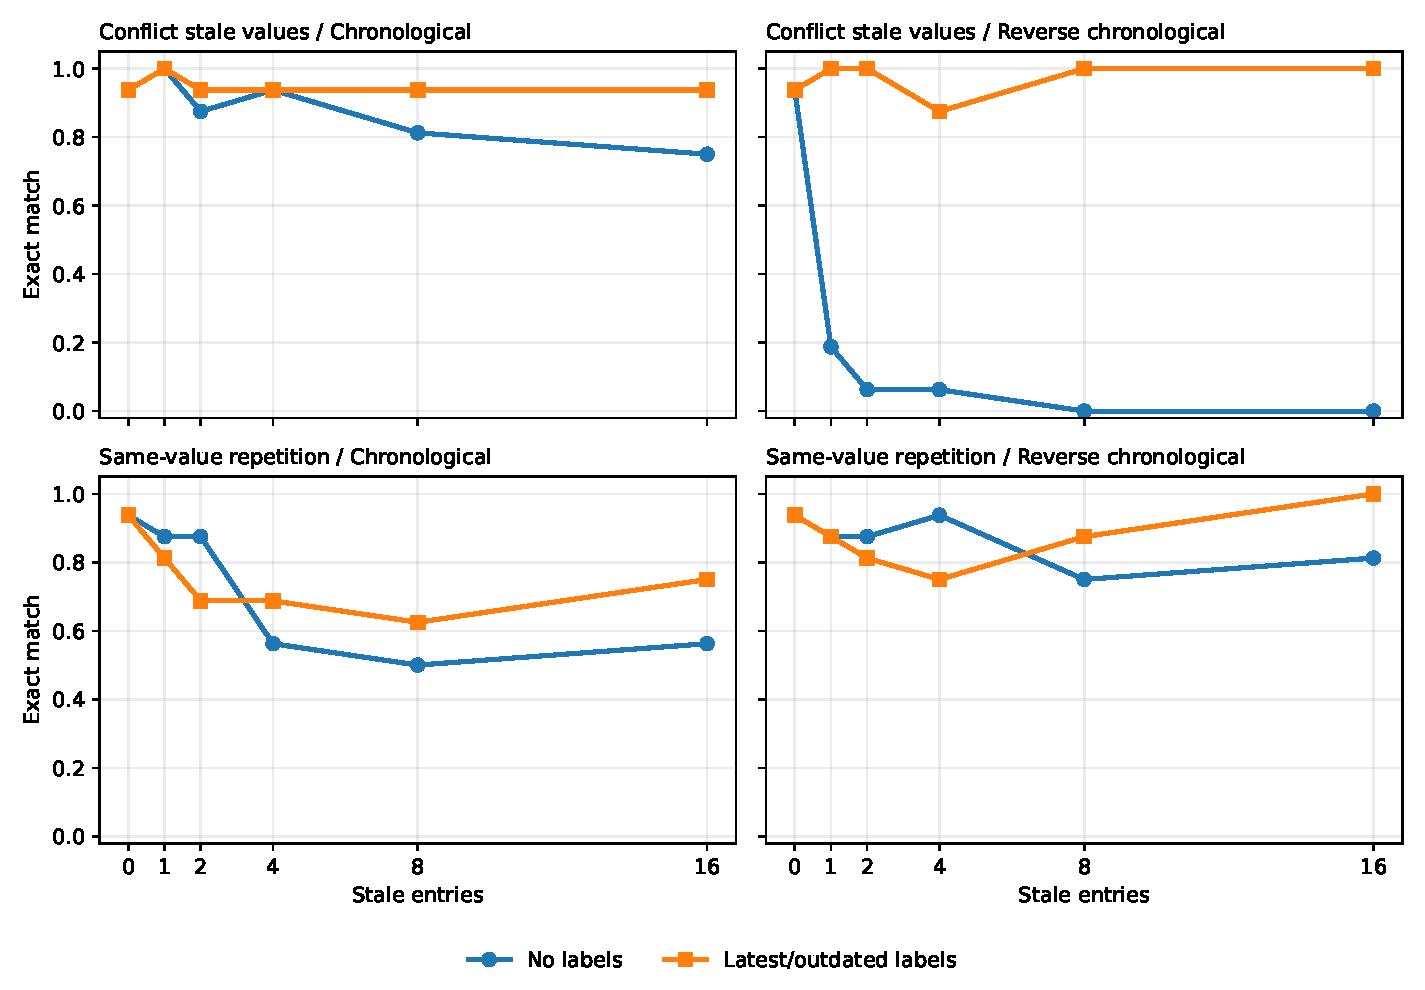
\includegraphics[width=\linewidth]{figures/p80_synthetic_same_slot_matrix.pdf}
  \caption{Synthetic same-slot probes (64 examples per cell). Conflicting stale values in reverse chronological order collapse EM rapidly; explicit version labels almost fully repair the failure. Same-value repetition still reduces exact EM despite answer-value-present staying at 1.0.}
  \label{fig:synthetic-same-slot}
\end{figure}

Figure~\ref{fig:synthetic-same-slot} reveals a clear decomposition:

\paragraph{Value conflict drives the sharpest collapse.}
With conflicting stale values in reverse chronological order (current value buried under obsolete ones), a single stale entry drops EM to 0.234, and two stale entries push it to 0.094.  At 8--16 stale entries, EM reaches the floor.

\paragraph{Majority voting is not the full story.}
If the model simply voted for the most frequent value, chronological order should not matter---but it does.
With conflicting values in \emph{chronological} order (current value last), EM remains 0.797 even at stale=16.
The model uses recency, not frequency.

\paragraph{Version labels repair the failure.}
Adding explicit \texttt{[latest]}/\texttt{[outdated]} labels to the reverse-chronological conflict condition raises EM from near zero to 0.969--1.000 across all stale counts.
The model \emph{can} handle stale context when version status is unambiguous.

\paragraph{Same-value repetition has a separate effect.}
When stale entries repeat the current value, answer-value-present stays 1.000 but exact EM drops (0.688 at stale=4, 0.531 at stale=16).
This indicates a formatting-dilution or attention-spreading effect that is independent of value conflict.

\subsection{Position sensitivity}
\label{sec:position-probe}

The chronological-order advantage suggests a recency bias: the model preferentially attends to entries near the end of the context.
We test this directly with a Lost-in-the-Middle-style probe~\citep{lost_in_the_middle}: holding the context set fixed, we vary only the \emph{position} of the gold (current-value) entry among stale entries.

\begin{table}[t]
\centering
\small
\begin{tabular}{lrrr}
\toprule
Gold position & EM & F1 & Ans.\ value \\
\midrule
Beginning & .010 & .073 & .040 \\
Middle    & .090 & .183 & .190 \\
End       & .630 & .654 & .720 \\
\bottomrule
\end{tabular}
\caption{Lost-in-the-Middle gold-position probe (\(k{=}16\) dev, Qwen). Moving only the gold entry's position among identical stale context. Final position yields 63$\times$ the EM of the beginning position.}
\label{tab:litm-probe}
\end{table}

Table~\ref{tab:litm-probe} confirms a strong \emph{monotonic} recency advantage: gold at the end yields 0.630~EM, in the middle 0.090, and at the beginning 0.010.
Unlike the U-shaped curve reported for long-context retrieval~\citep{lost_in_the_middle}, stale-contaminated short contexts show a purely recency-dominated pattern---the model almost never recovers a value buried under stale entries.

This explains the synthetic-probe results: chronological order naturally places the current value last (high recency), while reverse chronological buries it first (low recency).

\subsection{Dose--response}
\label{sec:dose-response}

Finally, we quantify how much stale exposure is needed to trigger collapse.
Pooling raw-append \texttt{slot\_prompt} runs across all \(k\) levels, we bin examples by their stale same-slot count.

\begin{figure}[t]
  \centering
  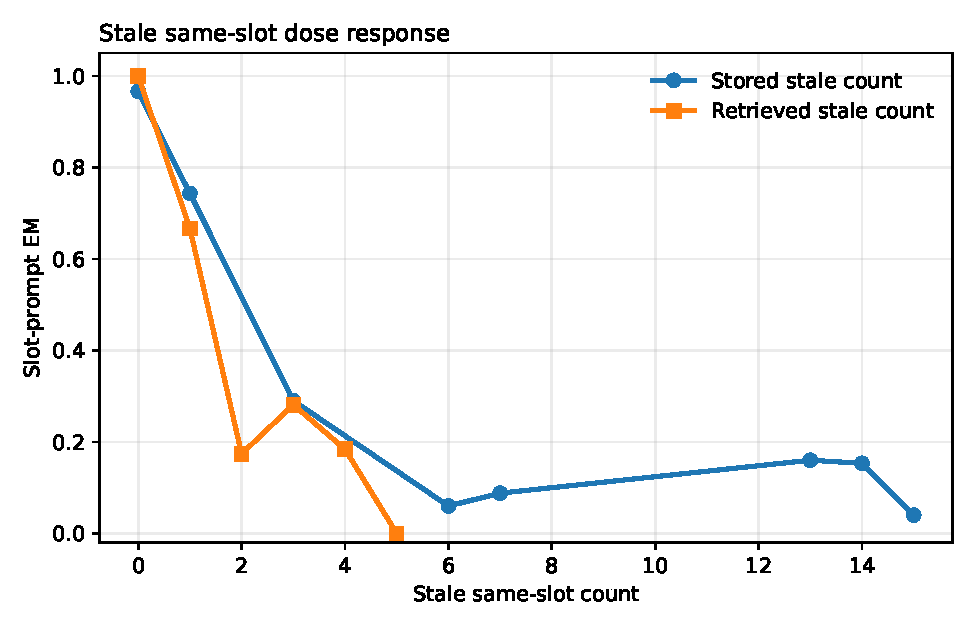
\includegraphics[width=\linewidth]{figures/p80_stale_dose_response.pdf}
  \caption{Dose--response: EM drops sharply with stale exposure. Retrieved stale count has a steeper slope and lower ED50 than stored stale count, supporting an answer-context exposure mechanism.}
  \label{fig:stale-dose-response}
\end{figure}

EM drops from 0.967 with zero stored stale entries to 0.743 with one and 0.290 with three (Figure~\ref{fig:stale-dose-response}).
A lightweight logistic fit estimates ED50 at 3.18 stored stale entries versus 1.89 \emph{retrieved} stale entries, confirming that answer-context exposure is the proximate mechanism: it is not how many stale entries exist in memory, but how many reach the answer prompt.

% ============================================================
% §6  ERROR ANALYSIS AND RESIDUAL LIMITS
% ============================================================
\section{Error Analysis and Residual Limits}

The ceiling-recovery and mechanism results show that stale context is the dominant \emph{stale-specific} obstacle.
But perfect stale removal does not yield perfect answering: Constrained CRUD reaches state accuracy 1.00 and zero stale entries at \(k{=}16\), yet its \texttt{slot\_prompt} EM remains 0.70.
The 0.30 residual reflects clean-context answer-layer limits---prompt-following failures, attribute-parsing errors, and generation noise---rather than stale contamination.

The three-model comparison sharpens this point: Llama's clean-context ceiling (0.27) is far below Qwen's (0.70) and Mistral's (0.72), even though all three have identical memory state.
These differences are instruction-following gaps, not stale-mechanism differences.

Long25 illustrates the complementary failure mode.
It greatly reduces stale burden (1.13 vs.\ 14.25 for Raw append) and memory size (9 vs.\ 52), but its \(k{=}16\) state accuracy is 0.91 rather than 1.00.
Error analysis shows these are primarily \emph{wrong final values} under hard distractors rather than wrong-entity or wrong-attribute failures: the learned manager sometimes over-compacts and drops the latest update.
This supports a compactness--reliability interpretation: learned compaction removes stale evidence but must still preserve the latest value exactly.

% ============================================================
% §7  RELATED WORK
% ============================================================
\section{Related Work}

\paragraph{Long-term memory benchmarks.}
LoCoMo~\citep{locomo} and LongMemEval~\citep{longmemeval} evaluate whether LLM agents can recall facts from long conversational histories.
They test memory \emph{existence}---can the system remember that a fact was stated?
MemUpdateBench tests memory \emph{hygiene}---when the same fact is revised repeatedly, do obsolete versions persist and interfere?
This is a complementary failure mode that broad benchmarks can miss because they typically use each fact only once.

\paragraph{External memory systems.}
Systems such as MemGPT~\citep{memgpt} and Mem0~\citep{mem0} operationalize persistent memory in agent workflows, providing the practical motivation for our benchmark.
They are \emph{systems} that must solve many problems simultaneously (retrieval, summarization, scheduling); MemUpdateBench is a \emph{diagnostic tool} that isolates one stressor.
We do not claim to benchmark these systems fairly; instead, we provide a transparent extract-then-store diagnostic pipeline that reproduces the stale-collapse and stale-filtering phenomena with inspectable memory state.

\paragraph{Knowledge editing.}
Knowledge editing methods modify model parameters to update specific facts~\citep{knowledge_editing_survey, mquake}.
The failure mode is different: editing suffers from \emph{ripple effects} where changing one fact unintentionally alters related knowledge, while external-memory update suffers from \emph{stale contamination} where old values persist alongside new ones.
MemUpdateBench studies the latter via inspectable external memory rather than opaque parametric edits.

\paragraph{Dialogue state tracking.}
Dialogue state tracking (DST) maintains slot--value states across conversation turns~\citep{dst_survey}.
MemUpdateBench borrows DST's diagnostic clarity---exact slots with known gold values---while shifting the focus to \emph{external memory persistence}: the question is not only whether the current state is correct, but whether obsolete values remain in memory and later interfere with answering.

\paragraph{Long-context position bias.}
\citet{lost_in_the_middle} show that LLMs underuse information in the middle of long contexts, producing a U-shaped accuracy curve.
Our Lost-in-the-Middle probe (\S\ref{sec:position-probe}) reveals that in \emph{short but stale-contaminated} contexts the pattern is different: accuracy drops monotonically from end to beginning, with no primacy recovery.
This suggests that stale same-slot entries create a stronger interference signal than mere positional distance.

% ============================================================
% §8  DISCUSSION AND LIMITATIONS
% ============================================================
\section{Discussion and Limitations}
\label{sec:limitations}

\paragraph{Design implications.}
The central finding is a tradeoff curve, not a method ranking.
Append-only memory preserves final values under oracle lookup but accumulates stale evidence that breaks prompted answering.
Heuristic compaction reduces growth but leaves enough stale entries to cause severe degradation.
Learned compact managers reduce stale burden but risk dropping the latest value.
The stale-filtering intervention shows that removing obsolete entries at retrieval time is sufficient to restore each model to its own ceiling.

This has a concrete design implication: \emph{memory systems that accumulate evidence without version management will fail under repeated updates, regardless of the answer model's capability.}
The mechanism analysis further shows that the failure can be partially mitigated by context presentation (chronological ordering, explicit version labels), but retrieval-time stale removal is the most effective single intervention.

\paragraph{Limitations.}
MemUpdateBench uses synthetic slot-structured examples rather than unconstrained real user histories, because the goal is to isolate repeated same-slot update behavior and measure stale burden exactly.
Real memory systems face noisier language, implicit updates, uncertain entity boundaries, and facts whose attributes are not named explicitly.

The current comparison does not include a fair evaluation of external memory SDKs.
We include a transparent diagnostic pipeline with inspectable records rather than an ecosystem benchmark, and we acknowledge this gap.

The benchmark stops at \(k{=}16\) because this level already separates oracle recoverability from prompted answer robustness decisively; higher-frequency stress points can be added if needed.

The current work contributes the benchmark, diagnostic decomposition, and evidence chain rather than a repaired method.
Long25 should be read as a checkpoint illustrating the compactness--reliability tradeoff, not as evidence that repair training has solved repeated same-slot updates.

% ============================================================
% REPRODUCIBILITY
% ============================================================
\paragraph{Reproducibility.}
Code, data, and canonical regeneration commands will be released upon acceptance.
All manuscript numbers trace to versioned result artifacts through a claim--evidence matrix included in the supplementary material.

\bibliography{references}
\bibliographystyle{plainnat}

\end{document}
